% !TEX encoding = UTF-8 Unicode

\documentclass[a4paper]{article}

\usepackage{color}
\usepackage{xcolor}
\usepackage{url}
\usepackage[T2A]{fontenc} % enable Cyrillic fonts
\usepackage[utf8]{inputenc} % make weird characters work
\usepackage{graphicx}
\usepackage{amsthm}
\usepackage{amsmath}

%\usepackage[english,serbian]{babel}
\usepackage[english,serbianc]{babel} %ukljuciti babel sa ovim opcijama, umesto gornjim, ukoliko se koristi cirilica

\usepackage[unicode]{hyperref}
\hypersetup{colorlinks,citecolor=green,filecolor=green,linkcolor=blue,urlcolor=blue}

\newtheorem{primer}{Пример}[section] %ćirilični primer
%\newtheorem{primer}{Primer}[section]

\newtheorem{definic}{Дефиниција}
\newcommand{\norm}[1]{\left\lVert#1\right\rVert}

\begin{document}

%TODO smisliti naslov
\title{Примена машинског учења у статичкој верификацији софтвера\\ \small{Семинарски рад у оквиру курса\\Методологија стручног и научног рада\\ Математички факултет}}

\author{Лазар Ранковић, Немања Мићовић, Урош Стегић\\ lazar.rankovic@outlook.com, nmicovic@outlook.com, mi10287@alas.matf.bg.ac.rs}
\date{}
\maketitle

\abstract{
%U ovom tekstu je ukratko prikazana osnovna forma seminarskog rada. Obratite pažnju da je pored ove .pdf datoteke, u prilogu i odgovarajuća .tex datoteka, kao i .bib datoteka korišćena za generisanje literature. Na prvoj strani seminarskog rada su naslov, apstrakt i sadržaj, i to sve mora da stane na prvu stranu! Kako bi Vaš seminarski zadovoljio standarde i očekivanja, koristite uputstva i materijale sa predavanja na temu pisanja seminarskih radova. Ovo je samo šablon koji se odnosi na fizički izgled seminarskog rada (šablon koji \emph{morate} da ispoštujete!) kao i par tehničkih pomoćnih uputstava. Molim Vas da kada budete predavali seminarski rad, imenujete datoteke tako da sadrže temu seminarskog rada, kao i imena i prezimena članova grupe (ili samo temu i prezimena, ukoliko je sa imenima predugačko). Predaja seminarskih radova biće isključivo preko web forme, a NE slanjem mejla.
Верификација софтвера постаје све битнија дисциплина (реф). Класични приступи су добри, имају супер резултате (реф). Машинско учење постаје све популарније. Показаћемо преглед радова који примењују алгоритме машинског учења у циљу убрзања процеса верификације (реф).
%Пошто ћемо абстракт писати на крају, онда док радимо да искористимо
%ово за интерне потребе. До сада прегледани радови:\\
%\begin{itemize}
%   \item{Finding latent code errors via machine learning over program executions
%       \cite{Brun04findinglatent}}
%   \item{Learning Invariants using Decision Trees
%       \cite{KrishnaPW15}}
%   \item{ICE: A Robust Framework for Learning Invariants
%       \cite{Garg2014}}
%   \item{Interpolants as Classifiers
%       \cite{Sharma_interpolantsas}}
%   \item{Advanced Verification Techniques Based on learning
%       \cite{Jain}}
%   \item{A Survey of Static Program Analysis Techniques
%       \cite{survey}}
%   \item{A Survey of Automated Techniques for Formal Software Verification
%       \cite{dkw2008}}
%   \item{Regresiona verifikacija softvera korišćenjem sistema LAV
%       \cite{milena}}
%\end{itemize}

\tableofcontents

\newpage

% ---------------------------------------------------------------------------------------------------------------------
\section{Uvod}
% ---------------------------------------------------------------------------------------------------------------------
Увод ћемо пред крај писати.

% ---------------------------------------------------------------------------------------------------------------------
\section{Верификација софтвера}
% ---------------------------------------------------------------------------------------------------------------------

\emph{Верификација софтвера} је дисциплина развоја софтвера која за циљ има провераву да ли програм задовољава све унапред задате захтеве. Ти захтеви су представљени спецификацијом свих жељених особина програма и дефинишу се пре процеса верификације. Највећа примена верификације софтвера је у оптимизацији кода и провери исправности.


Потребно је направити разлику између тоталне и делимичне исправности. Испитивање тоталне исправности захтева да се за све могуће улазе покаже заустављање програма. Доказ заустављања у општем случају није могуће извести \cite{turing}. Такође, испитивање нетривијалних семантичких својстава је неодлучив проблем \cite{rice}. Према томе, у рачунарству је довољно испитати делимичну исправност софтвера, тј. довољно је показати да ће резултат извршавања програма бити валидна вредност.


Два приступа при верификацији софтверa су \emph{динамичка верификација} и \emph{статичка верификација} \cite{milena} 
\begin{itemize}
\item \textbf{Динамичка верификација}\\
Овај вид верификације се врши у току извршавања програма и то најчешће скупом 
унапред припремљених тестова који морају бити испуњени. Очигледно је да због неисцрпне варијације могућих улаза, овај вид тестирања нема за циљ валидацију програма, већ је циљ динамичке верификације проналажење грешка на неком не тривијалном скупу тестова.
\item \textbf{Статичка верификација}\\
Статичка верификација софтвера подразумева анализу софтвера без његовог извршавања, тачније анализу кода применом неке од технника које ће бити описане у наставку. Анализу кода може обављати човек, а може се и аутоматизовати. Аутоматизација подразумева описивање (па чак и превођење) кода језиком изабране математичке теорије.
\end{itemize}


У наставку ће бити више речи о статичкој верификацији. Биће описани механизми анализе кода, технике верификације и чести проблеми овог типа верификације.
% ---------------------------------------------------------------------------------------------------------------------
\section{Технике статичке верификације}
% ---------------------------------------------------------------------------------------------------------------------
Претходним поглављем су дефинисани основни појмови верификације софтвера. Предочено је да је немогуће у општем случају испитати заустављање програма и анализирати нетривијална семантичка својства. Ово поглавље ће дати увид у аутоматизоване технике статичке анализе.

\subsection{Апстрактна интерпретација}
Апстрактна интерпретација је теорија семантичке апроксимације чија је идеја да изгради нову семантику над програмским језиком тако да се конкретан програм увек завршава. Тако се анализа програма врши над апстрактном семантиком да би се добила апроксимација над целом семантиком. Коришћење апстрактне интерпретације се омогућава помоћу две функције: функције која пресликава конкретне вредности у апстрактне вредности и функције која слика апстрактне вредности у конкретне вредности. Неизбежно је заобићи губљење података при пресликавању из конкретних вредности у апстрактне вредности јер је циљ показати да се над апострактном семантиком програм завршава. Користећи овај математички оквир је релативно лако показати да ако се програм завршава у новој семантици програм ће бити коректан и у стварној семантици.


\subsection{Симболичкa анализа}
Симболичкa анализа је метод статичке анализе који анализира програмске вредности који могу да се мењају. Овај метод има за циљ да изведе математички модел који прецизно описује израчунавање, заправо може се посматрати као нека врста компајлера који преводи програм у симболичке изразе. Квалитет алгебарских система као што су (Axiom, Derive, Macsyma, Maple, Mathematica, MuPAD, and Reduce) је веома битан јер квалитет овог начина анализе у великој мерим зависи од паметних алгебарских упрошћавања.


\subsection{Проверавање ограничених модела}
\textit{Проверавање ограничених модела} (енг. Bounded model checking) је техника верификације која се највише користи у индустрији полуповодника, тачније верификација логичкх кола. Укратко речено смисао је да се логичка кола опишу исказном логиком. Следећи корак је провера задовољивости добијене исказне формуле. Испитивање задовољивости формула је НМ-тежак проблем, и за решавање овог питања користе се сат решавачи. Ефикасност сат решавача је од кључног значаја за ову технику. Ова техника је такође примењљива и за анализу софтвера, један од начина примене је посматрање извршавања целокупног програма као скупа стања, односно као један коначни аутомат у ком се прелази из стања у стање. Ако се тако посматра програм могуће је описати сва стања искасном логиком затим повезати сва стања и тако добијену формулу пустити у сат решавач. Резултат сат решавача је може бити формула је задовољива сто би значило да је програм коректан или ако је формула незадовољива резултат ће бити контрапример којим се показује да програм није коректан и може представљати основу за дебаговање.\cite{survey}\cite{dkw2008}.

Овим поглављем смо направили кратак преглед најважнијих техника аутоматизоване статичке анализе. Показује се да наведене
технике дају неку врсту формалне гаранције квалитета софтвера. Апстрактна семантика је уопштени начин рада кад се прави
програм за анализу софтверa, тако да се сви остали програми који спроводе анализу могу бити посматрани као инстанце апстрактне
семантике.  Симболичкa анализа је техника којом се изводи прецизна карактеризација програмских својстава на параметарски начин, а
техника проверавања ограничених модела је моћна за октривање једноставних грешака али на жалост нису у стању да
докажу чак ни дубоке петље. \\
У следећем поглављу ћемо објаснити основне аспекте области машинског учења.

% ---------------------------------------------------------------------------------------------------------------------
\section{Машинско учење}
% ---------------------------------------------------------------------------------------------------------------------
У претходним поглављима смо представили увод у статичку верификацију софтвера. Показана је важност те области и изложене су технике верификације. Овим поглављем ћемо представити област машинског учења. Описаћемо главне аспекте ове дисциплине, показаћемо њену битност и даћемо преглед важних концепата о којима ће бити више речи у поглављу 6.
%Овим поглављем ћемо дати одговоре на следећа питања:
%\begin{itemize}
%\item Шта је машинско учење?
%\item У чему је значај ове области?
%\item Основни принципи.
%\end{itemize}

\subsection{Основе машинског учења}
\begin{definic}
%A computer program is said to learn from experience E with respect to some class of tasks T and performance measure P if its performance at tasks in T, as measured by P, improves with experience E.
``За програм кажемо да учи из искуства E кроз обављање задатка T са мером квалитета P, ako повећањем искуства E расте мера P за обављен задатак T.''
\\[5pt]
\rightline{{\rm --- Tom M. Mitchell} \cite{tom-ml}}
\end{definic}


Машинско учење можемо посматрати као област рачунарства која се бави анализом алгоритама који генерализују. Са практичног аспекта, генерализација може значити уопштавање закона над датим подацима.


Машинско учење се дели на три подобласти: \textit{надгледано учење}, \textit{ненадгледано учење} и \textit{учење условљавањем}. Подаци из којих алгоритми машинског учења уче, могу бити обележени, необележени и могу се генерисати у фази учења. Оваква природа података је основ за разликовање три наведене подобласти.\cite{tom-ml}.


Међу многим проблемима над којима су често примењивани алгоритми машинског учења, издвојићемо проблем регресије и проблем класификације. Ови проблеми су релевантни за теме којих ћемо се дотаћи у овом раду. Под проблемом класификације подразумевамо испитивање инстанце датог објекта и одређивање класе којој он припада на основу његових својстава (атрибута). Типичан пример класификације је одређивање порекла тумора (испитивање да ли је тумор малигни или бенигни) на основу његове величине. Проблем регресије представља предикцију неког параметра популације за дати објекат на основу осталих атрибута тог објекта. Као пример можемо узети предикцију цене стамбеног објекта на основу његове величине, броја соба и разних других релевантних карактеристика.


Пре примене машинског учења потребно је проучити проблем који се решава, уочити његове специфичности и припремити и анализирати податке из којих ће алгоритми учити. Након детаљне анализе, врши се одабир одговарајућег математичког модела који ће нам дати одговор на проблем који решавамо. Када смо изабрали модел, вршимо његово тренирање на инстанцама припремљених података. Тренинг радимо тако што довољан број пута пуштамо модел да решава наш проблем и меримо успешност тј. грешку коју тај модел прави. Након сваког мерења, у зависности од алгоритма који примењујемо, вршимо корекцију модела у циљу минимизације грешке.


Општи опис који смо сада представили ће у даљем тексту бити детаљније образложен. Приказаћемо конкретне алгоритме и дискутовати о њиховим својствима. Алгоритме које ћемо посматрати су од велике важности за примену у статичкој верификацији, па је с тога важно њихово потпуно разумевање. Пре него што дамо преглед тих алгоритама, покушаћемо да приближимо значај машинског учења уопштено као и његов значај у статичкој верификацији.


\subsection{Значајност машинског учења}
Конвенционалан начин решавања проблема у рачунарству се своди на формално дефинисање низа корака који улазне параметре трансформишу не би ли дошли до резултата. Овакав приступ је користан у ситуацијама када је потребно решити проблеме који су човеку изазовни, као што су компликоване рачунске операције, сортирање великих низова и томе слично. Поставља се питање: како написати програм који би обављао задатке које човек свакодневно лако обавља? На пример, да ли је могуће написати програм који би био у стању да препознаје објекте са фотографија?


\textit{Рачунарски вид} (енг. computer vision) је дисциплина која се бави овим проблемом.\cite{old-cv}. Алгоритми који су примењивани пре раста популарности машинског учења нису показали значајне резултате. Могли су да генеришу једноставне геометријске моделе који нису давали задовољавајуће резултате. Дубоке неуронске мреже су алгоритами машинског учења који су показали значајне напретке у овој области \cite{new-cv}.


Класификација дела програма на валидна стања и она која могу резултовати грешком је од кључног значаја за ефикасност алата за верификацију \cite{Brun04findinglatent} \cite{KrishnaPW15}. Конкретним проблемима и њиховим решењима ћемо се бавити у наредним поглављима.


\subsection{Технике машинског учења}
Оптшу слику о томе како се примењују алгоритми машинског учења смо дали у уводном делу овог поглавља. Сада ћемо видети неке конкретне алгоритме и њихове особине. Како је проблем класификације централни проблем над којиме се примењује машинско учење у статичкој верификацији, описаћемо два алгоритма који решавају тај проблем. Зарад потпуности, описаћемо и један алгоритам решавања регресионих проблема.


\subsubsection*{Линеарна регресија}
Као што је речено у уводном делу, регресиони проблем представља предвиђање циљне променљиве непознате инстанце на основу осталих њених атрибута. Означимо са $y_i$ циљну променљиву, а са $\vec{x} = (x_1, x_2, ..., x_n)$ вектор атрибута које посматрамо. У примеру предикције вредности куће то могу бити број соба, квадратура куће итд. Инстанцу из скупа података онда представљамо уређеним паром $(\vec{x}_i, y_i)$. Модел линеарне регресије, параметризован вектором $w$, који описује законитост је следећи:
\begin{equation}
    h(\vec{x}_i) = w^T \cdot \vec{x}_i
\end{equation}


Грешка коју модел прави можемо представити погодним избором функције грешке $L(w)$. Чест избор ове функције је средњеквадратна грешка коју модел прави над свим инстанцама из тренинг скупа.
\begin{equation}
L(w) = \frac{1}{N}\sum \limits_{i=1}^{N} (h(\vec{x}_i) - y_i)^2
\end{equation}

Тренинг вршимо тако што одређеном оптимизационом техником вршимо минимизацију функције грешке по параметрима $w$.


\subsubsection*{Стабла одлучивања}
Стабла одлучивања представљају један од основних метода класификације. Употребу стабала одлучивања оправдава њихова висока интерпретабилност \cite{dct-survey}. У листовима стабла одлучивања се налазе вредности циљне променљиве, односно у случају класификације, класе којима инстанца може припасти. Чворови стабла представљају атрибуте по којима се врши подела. Када су ти атрибути категоричког типа, потомци датог чвора су добијени из свих могућих вредности које тај категорички атрибут може имати. У случају да је атрибут некатегоричког типа, најчешће се врши подела могућих вредности на дисјунктне интервале тако да свако дете тог чвора одговара једном од интервала. Слика \ref{fig:stablo} приказује једно могуће стабло одлучивања добијено на основу података.

\begin{figure}[h!]
\begin{center}
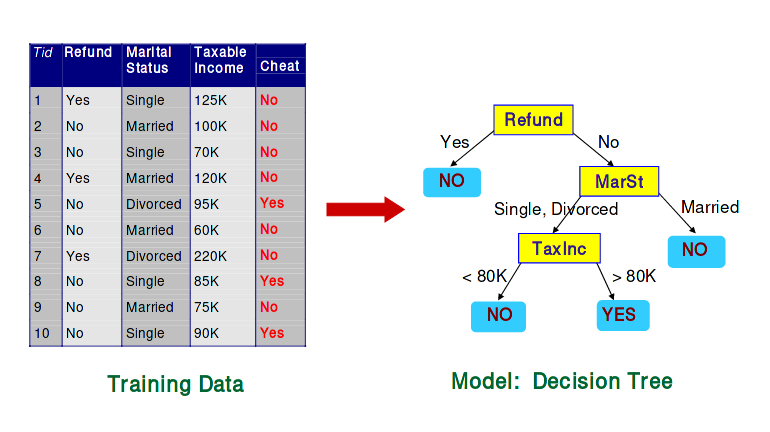
\includegraphics[scale=0.4]{decision_tree.png}
\end{center}
\caption{Стабло одлучивања}
\label{fig:stablo}
\end{figure}


\subsubsection*{Метода потпорних вектора}
Проблем класификације можемо посматрати на следећи начин. Инстанце које класификујемо представљамо тачкама у неком високодимензионалном простору. Бинарни класификатор који тренирамо је хиперраван која дели простор на два дела, тако да се у једном делу простора нађу све инстанце које припадају једној класи, а у другом делу ће се наћи оне које припадају другој класи. Раздвајајућих хиперравни може бити више, па је зато потребно одабрати хиперраван која боље описује поделу међу подацима \cite{svm-intro}.


Маргина класификације је најмање растојање између тачака које се налазе у различитим потпросторима. Слика \ref{fig:svm} приказује хиперравни $B_1$ и $B_2$. Интуитивно видимо да ће прва хиперраван боље раздвојити податке. Маргина $(b_11, b_12)$ je значајно већа од маргине $(b_{21}, b_{22})$ и то је оно што први класификатор чини знатно бољим.

\begin{figure}[h!]
\begin{center}
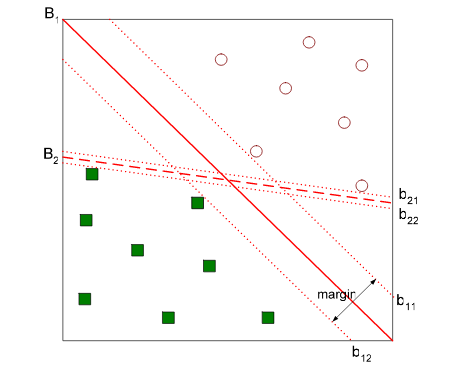
\includegraphics[scale=0.6]{svn.png}
\end{center}
\caption{Приказ различитих хиперравни}
\label{fig:svm}
\end{figure}

Максимизацијом маргине добијамо класификатор који боље описује поделу. Зарад конвенције, проблем максимизације сводимо на проблем минимизације, те добијамо следећи оптимизациони проблем:
\begin{equation}
    \min_{w, w_0} \frac{ {\norm{w}}^2 }{2}
\end{equation}


Пошто смо видели основне алгоритме машинског учења, у следећем поглављу ћемо описати везу измећу статичке верификације и машинског учења. Бавићемо се проблемима статичке верификације који су погодни за решавање техникама машинског учења.


% ---------------------------------------------------------------------------------------------------------------------
\section{Одабрани проблеми статичке верификације}
% ---------------------------------------------------------------------------------------------------------------------
%\textit{Уређени бинарни дијаграми одлучивања} (енг. ordered binary decision diagrams, OBDD) \cite{obdd} представљају алат за ефикасну анализу Булових функција.\cite{eval-obdd}\cite{logic-ver-synth}. Логичке импликације бивају откривене конструисањем УБДО за разне улазе. Симболичком обрадом УБДО дијаграма и применом закона контрапозиције се могу научити додатне импликације. \cite{Jain}. Статичка верификација се даље спроводи успостављањем еквиваленције између два УБДО, тј. проналаском одговарајућег скупа импликација. Еквивалентност два УБДО се изводи проналажењем сличности унутрашње структуре између два дијаграма.
До сада смо видели стандардне проблеме и технике статичке верификације и машинског учења. У овом поглављу ћемо издвојити значајне проблеме верификације на које су, применама алгоритама машинског учења постигнути значајнији резултати.


Статичка верификација мора бити у стању да разликује позитивна стања програма од негативних.
Негативна су она која доводе програм до грешке. \textit{Интерполантама} (енг. interpolants)
називамо предикате који раздвајају позитивна од негативних стања.
У статичкој верификацији се коришћењем оваквих интерполанти гради даљи доказ.
Показано је да се ове интерполанте могу интерпретирати као бинарни класификатори.
Проблем који се овде јавља је генерисање интерполанти, тј проналажење одговарајућег класификатора \cite{Sharma_interpolantsas}.
У делу  \ref{ssec:interpolant} детаљније је описан приступ коришћен у \cite{Sharma_interpolantsas}.

Поред итерполанти, могуће је препознати нетривијална својства програма која даље резултују грешком.
Грађењем \textit{класификатора нетачне инваријанте} (енг. False Invariant Classifier) је могуће рангирати
својства програма по томе колику вероватноћу за грешком та својства проузрокују.
Одређивање нетривијалног својства датог програма је у општем случају неодлучив проблем \cite{turing, Brun04findinglatent}.

Код апстрактне интерпретације је остварив баланс између прецизности изгенерисане инваријанте и скалабилности система за верификацију. Овај баланс је последица детаљне анализе апстрактног синтаксног стабла. Одабир инваријанте је тежак проблем и показано је да се може утврдити тестирањем \cite{Sharma_interpolantsas, KrishnaPW15}.

Проблеми које смо представили овим поглављем су решена користећи одговарајуће технике машинског учења. У наредом поглављу ћемо се бавити тим решењима, даћемо увид у начине на који су та решења примењена и покушати да одговоримо на питање како наставити усавршавање тих техника.

% ---------------------------------------------------------------------------------------------------------------------
\section{Неке примене техника машинског учења у статичкој верификацији}
% ---------------------------------------------------------------------------------------------------------------------
\color{blue}
Ово је есенција. Одабирају се проблеми из претходног поглавља и показује се
како се решава. Прво иде неки уводни део, онда из литературе се покупе те технике
и таксативно се наводе (принцип проблем-решење).
\color{black}
\subsection{Проналажење интерполанти}
\label{ssec:interpolant}

Неформално говорећи, интерполанта представља предикат који раздваја позитивна стања програма
од негативних. Примена машинског учења у проналажењу интерполанти огледа се у добијању модела
који представља саму интерполанту. У делу \ref{sssec:interpolant_svm} изложене су основе из \cite{Sharma_interpolantsas} базиране на методу
потпорних вектора, док је у делу \ref{sssec:interpolant_dt} изложен приступ из рада \cite{KrishnaPW15} базиран на стаблима одлучивања. Експериментални резултати
показали су да приступи базирани на машинском учењу јесу упоредиви са традиционалним техникама.

%Користи се теорија линеарне аритметика о којој се више може пронаћи у \cite{Kroening2008}.

\subsubsection{Проналажење интерполанти користећи метод потпорних вектора}
\label{sssec:interpolant_svm}

Нека су $A$ и $B$ формуле у теорији линеарне аритметике \cite{Kroening2008}.
\begin{equation}
\phi ::= w^Tx + d \geq 0 \ | \ true \ | \ false \ | \ \phi \land \phi \ | \ \phi \lor \phi \ | \ \neg \phi
\end{equation}
При чему је $\vec{w} = (w_1, ..., w_n)^T \in R^n$ вектор константи у простору $R^n$; $\vec{x} = (x_1, ..., x_n)^T$
вектор променљивих из простора $R^n$.

\begin{definic}
Интерполанта за пар формула (А, B) тако да $A \land B \equiv \bot$ је формула I која задовољава $A \Rightarrow I, I \land B \equiv \bot$
при чему формула I садржи само променљиве које се јављају у формулама A и B.
\end{definic}

На слици \ref{fig:interpolant_example} приказан је програмски код који ће бити корићен као илустрација.
Функција непознат број пута инкрементира променљиве $x$ и $y$, потом их декрементира све док променљива $x$
не постане 0. Коначно, уколико је $y \neq 0$ онда програм одлази у стање грешке.
Приметимо да је инваријанта $x = y$ довољна да се докаже да програм никад неће доћи у стање грешке.

\begin{figure}[h!]
\begin{center}
    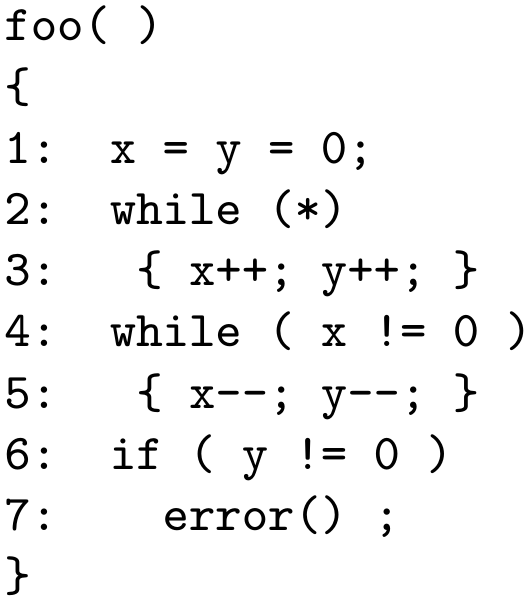
\includegraphics[scale=0.17]{./slike/interpolant_code.png}
\end{center}
\caption{Пример кода}
\label{fig:interpolant_example}
\end{figure}

Претпоставимо да је функцијa \texttt{foo()} извршила на следећи начин (у заградама су хронолошки наведени линије инструкција): $(1, 2, 3, 2, 4, 5, 4, 6, 7)$ који
води у стање грешке.  Поделимо ток на два скупа, A и B и пронађимо интерполанте за наведени ток.

Скуп A садржи вредности $x$ и $y$ које се добијају након извршавања линија 1, 2 и 3. У скупу B се налазе оне вредности $x$ и $y$
које би се добиле уколико би програм извршио линије 4, 5, 6 и 7 чиме би програм дошао у завршно стање.

Имамо да $A \land B \equiv \bot$ при чему важи:

\begin{equation*}
\begin{split}
    A & \equiv x_1 = 0 \land y_1 = 0 \land if\_then\_else(b,\  x = x_1 \land y = y_1,\ x = x_1 + 1 \land y = y_1 + 1)     \\
    B & \equiv if\_then\_else(x = 0,\ x_2 = x \land y_2 = y,\ x_2 = x - 1 \land y_2 = y-1) \land x_2 = 0 \land \neg (y_2 = 0)
\end{split}
\end{equation*}

$A$ представља скуп достижних стања док $B$ представља скуп стања која воде у стање грешке. Интерполанта је доказ да су
скупови $A$ и $B$ дисјунктни и изражава се користећи заједничке променљиве из скупова $A$ и $B$. Затим, помоћу доказивача теорема се рачунају вредности за $(x, y)$ које задовољавају формуле $A$ и $B$ \cite{Sharma_interpolantsas}.

Добијене вредности представљају скуп инстанци над којим се може тренирати класификациони модел (попут логистичке регресије или потпорних вектора).
Позитивне инстанце представљају вредности променљивих које задовољавају формулу $A$ и аналогно, негативне инстанце представљају вредности
променљивих које задовољавају формулу $B$.

\begin{figure}[h!]
\begin{center}
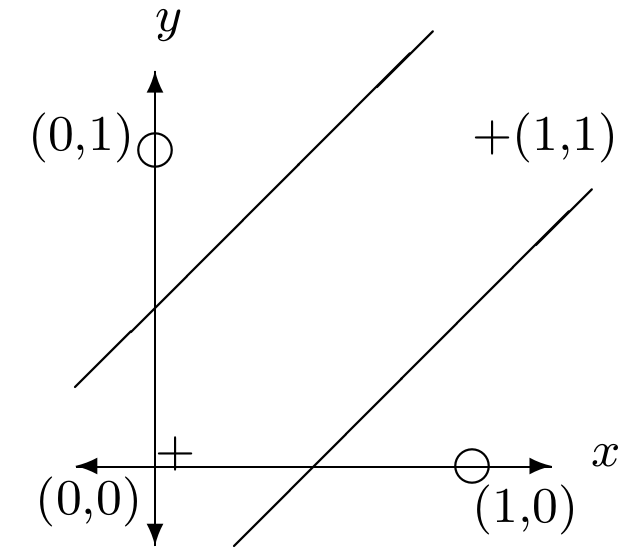
\includegraphics[scale=0.2]{./slike/interpolant.png}
\end{center}
\caption{Класификација у тражењу интерполанти}
\label{fig:interpolant_svm}
\end{figure}

Слика \ref{fig:interpolant_svm} приказује вредности променљивих $(x, y)$ за $A$ као плусеве (тачке $(0, 0)$ и $(1, 1)$)
и $B$ као кружиће (тачке $(1, 0)$ и $(0, 1)$). Приказани модел је добијен коришћењем метода потпорних вектора. Резултујуће праве одговарају једначинама:
\begin{equation*}
\begin{split}
    e_1: 2y &= 2x + 1 \\
    e_2: 2y &= 2x - 1
\end{split}
\end{equation*}
Интерполанта која се одавде може извести је
\begin{equation*}
2y \leq 2x + 1 \, \land 2y \geq 2x - 1
\end{equation*}

Овај предикат представља инваријанту чијим доказивањем се показује да програм не може доћи у стање грешке.
Једноставнија интерполанта $x = y$ се може добити транислирањем добијених правих што ближе позитивним истанцама,
докле год се одржава сепарабилност позитивних и негативних инстанци.

Табела \ref{table:interpolant_table} приказује резултате из \cite{Sharma_interpolantsas} на неким од познатих
примера. Интерполанте које су означене са \textit{исто} су интерполанте које су добијене користећи решавач \textsc{OpenSMT}.

\begin{table}[]
\centering
\caption{Добијене интерполанте на неким од познатијих тест примера у области.}
\label{table:interpolant_table}
\begin{tabular}{|c|c|l|}
\hline
\textbf{Датотека} & \textbf{Време (с)} 	& \textbf{Интерполанта}                                                     			\\ \hline
\texttt{f1a} 	& 0.022              	& \texttt{((y = 1 | x \textless= 0) \& x = 1) | (y = 0 \& (y = 1 | x \textless= 0))} 	\\ \hline
\texttt{ex1}    & 0.021              	& \texttt{xa + 2*ya >= 0 | xa + 2*ya >= 5 | xa + 2*ya >= 5}                             \\ \hline
\texttt{f2}     & 0.20               	& \texttt{y <= 3*x | y <= 3*x + 1 | y <= 3*x + 1} 										\\ \hline
\texttt{nec1}   & није доступно      	& Није пронађена                                                            			\\ \hline
\texttt{nec2}   & 0.018 				& \texttt{x < y} (исто) 																\\ \hline
\texttt{nec3}   & 0.016      			& \texttt{y <= 9} (исто)																\\ \hline
\texttt{nec4}   & 0.021      			& \texttt{(x = y | y = 0) | (y = x) | (y = x)} 											\\ \hline
\texttt{nec5}   & 0.018      			& \texttt{s >= 0} (исто) 																\\ \hline
\texttt{pldi08} & 0.017      			& \texttt{y > x}																		\\ \hline
\texttt{fse06}  & 0.017      			& \texttt{y + x >= 0 \& y >= 0 \& y >= 0 \& y >= 0}										\\ \hline
\end{tabular}
\end{table}

\subsubsection{Проналажење интерполанти користећи стабла одлучивања}
\label{sssec:interpolant_dt}

Интерполанте се могу извести и другим методима машинског учења. Рад \cite{KrishnaPW15} илуструје приступ који
користи стабла одлучивања. За програмски код се генеришу позитивне и негативне инстанце над којима се гради
стабло одлучивања користећи похлепни алгоритам. Правила добијена у стаблу се трансформишу у формулу која
се потом проверава да ли је инваријанта користећи \textsc{SMT} решавач.

Резултати су показали да једноставни похлепни алгоритам који гради стабло даје и једноставне формуле
за интерполанте. Стабло је лако научило комплексне бинарне инваријанте као једноставне коњункције.

Слика \ref{fig:interpolant_example2} приказује пример програма и његова стања која се могу добити на основу
покретања самог програма. Добра стања можемо добити пратећи претпоставке (линија 2), бележећи ток променљивих
и провером да ли је испуњен услов $x \neq 0$ са линије 12. Лоша стања можемо добити игноришући услов са линије 2.
На пример, тачка $(-2, -2)$ тачка $(-4, -4)$ представљају лоша стања.

\begin{figure}[h!]
\begin{center}
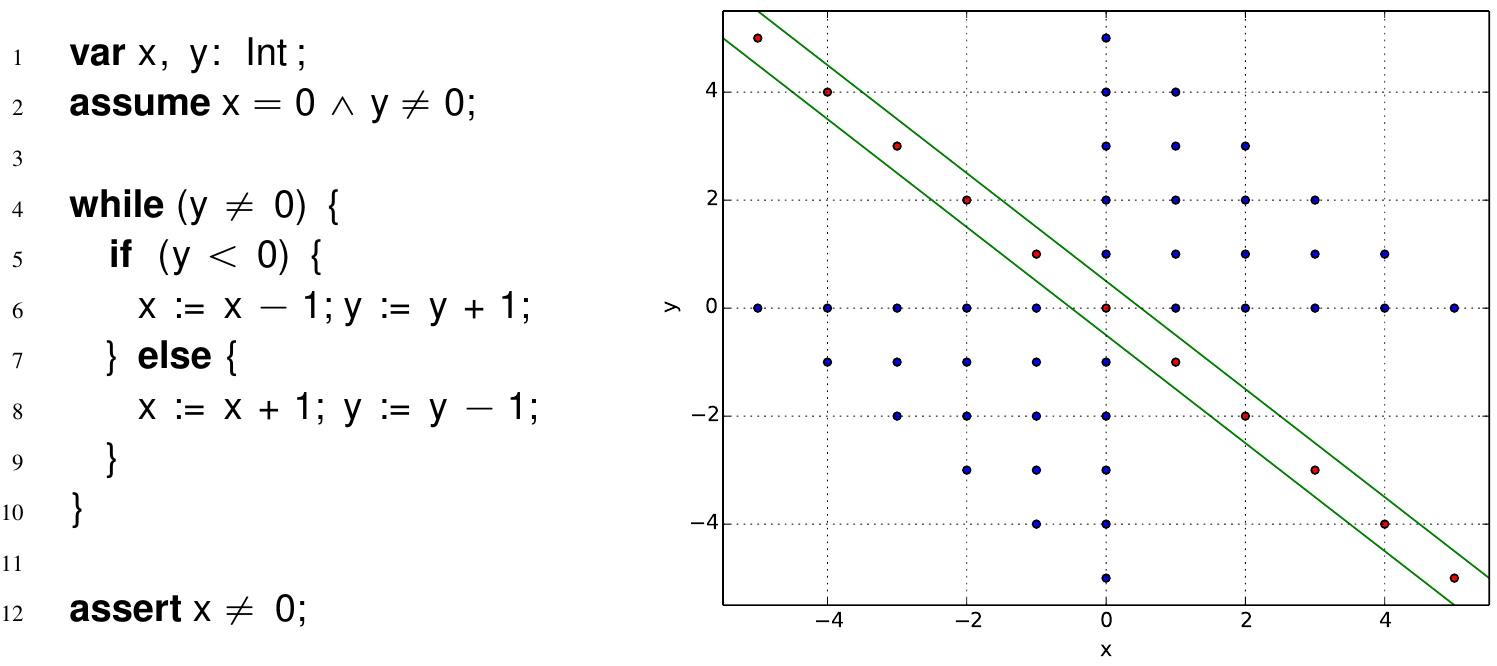
\includegraphics[scale=0.2]{./slike/interpolant2.png}
\end{center}
    \caption{Пример програма. Лева страна приказује код, десна страна садржи добра стања (плаве тачке) и лоша
    стања (црвене тачке).}
\label{fig:interpolant_example2}
\end{figure}

Слика \ref{fig:interpolant_dt} приказује стабло добијено применом алгоритма описаног у \cite{KrishnaPW15}.
Добијени алгоритам је сложености $O(mn \log(n))$, где је $m$ број атрибута а $n$ број инстанци.

\begin{figure}[h!]
\begin{center}
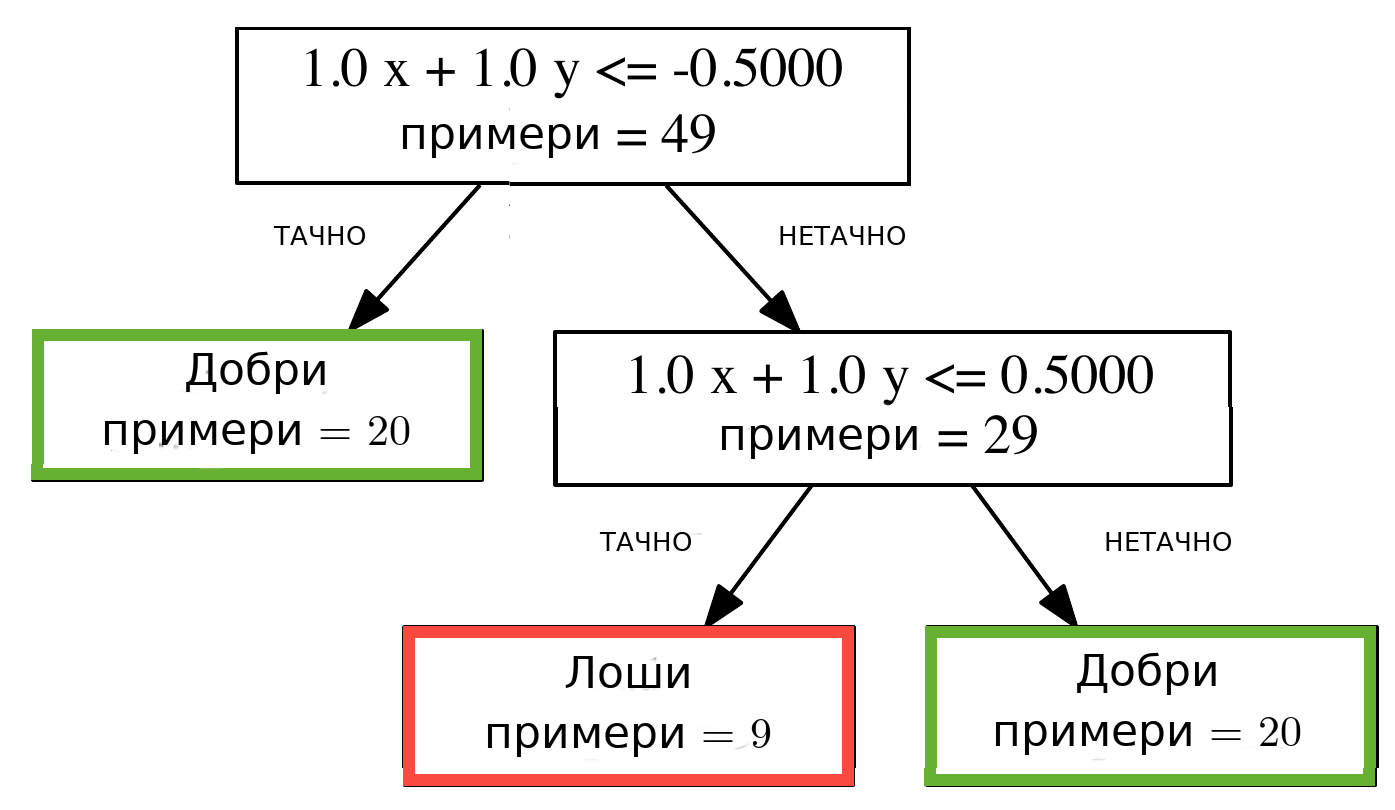
\includegraphics[scale=0.2]{./slike/stablo_odlucivanja.png}
\end{center}
    \caption{Стабло одлучивања добијено за пример са слике \ref{fig:interpolant_example2}.} 
\label{fig:interpolant_dt}
\end{figure}

\subsection{Грађење класификатора нетачне инваријанте}

% ---------------------------------------------------------------------------------------------------------------------
\section{Закључак}
% ---------------------------------------------------------------------------------------------------------------------
Овде машти на вољу.. :)


\addcontentsline{toc}{section}{Literatura}
\appendix
\bibliography{seminarski}
\bibliographystyle{plain}


\end{document}
